\ifx\wholebook\relax \else

\documentclass{article}

%
% loading packages
%

\RequirePackage{ifpdf}
\RequirePackage{ifxetex}

%
%
\ifpdf
  \RequirePackage[pdftex,%
       bookmarksnumbered,%
              colorlinks,%
          linkcolor=blue,%
              hyperindex,%
        plainpages=false,%
       pdfstartview=FitH]{hyperref}
\else\ifxetex
  \RequirePackage[bookmarksnumbered,%
               colorlinks,%
           linkcolor=blue,%
               hyperindex,%
         plainpages=false,%
        pdfstartview=FitH]{hyperref}
\else
  \RequirePackage[dvipdfm,%
        bookmarksnumbered,%
               colorlinks,%
           linkcolor=blue,%
               hyperindex,%
         plainpages=false,%
        pdfstartview=FitH]{hyperref}
\fi\fi
%\usepackage{hyperref}

% other packages
%--------------------------------------------------------------------------
\usepackage{graphicx, color}
\usepackage{wrapfig}
\usepackage{subfig}
\usepackage{multicol}
\usepackage{tikz}
\usetikzlibrary{matrix,positioning,shapes}
\usetikzlibrary{patterns}

\usepackage{amsmath, amsthm, amssymb} % for math
\usepackage{exercise} % for exercise
\usepackage{import} % for nested input

%
% for programming
%
\usepackage{verbatim}
\usepackage{fancyvrb}
\usepackage{listings}
%\usepackage{algorithmic} %old version; we can use algorithmicx instead
%\usepackage[plain]{algorithm} %remove rule (horizontal line on top/below the algorithm
\usepackage{algorithm} %to remove rules change to \usepackage[plain]{algorithm}
%\usepackage{algorithm2e}
\usepackage[noend]{algpseudocode} %for pseudo code, include algorithmicsx automatically
\usepackage{appendix}
\usepackage{makeidx} % for index support
\usepackage{titlesec}
\usepackage{epigraph}

\usepackage[cm-default]{fontspec}
\usepackage{xunicode}
%\usepackage{fontenc}
\usepackage{textcomp}
\usepackage{url}

% detect and select Chinese font
% ------------------------------
% fc-list :lang=zh    % list all Chinese fonts
% fc-list :mono       % list all mono fonts
% fc-cache            % refresh cache to load new installed fonts
\def\macmainfont{STSong}  % Under Mac OS X
\def\macmonofont{Monaco}
\def\winmainfont{SimSun} % Under Windows
\def\winmonofont{Consolas}
\def\linuxmainfont{WenQuanYi Micro Hei} % Under Linux
\def\linuxmainfont{Courier}

\suppressfontnotfounderror1 % Avoid setting exit code (error level) to break make process
\count255=\interactionmode
\batchmode

% main font
\let\mainft=\macmainfont
\font\thefont="\mainft"\space at 10pt
\ifx\thefont\nullfont
  \let\mainft=\winmainfont
  \font\thefont="\mainft"\space at 10pt
  \ifx\the\nullfont
    \let\mainft=\linuxmainfont
    \font\thefont="\mainft"\space at 10pt
    \ifx\the\nullfont
      \errorstopmode
      \errmessage{no suitable Chinese main font found}
    \fi
  \fi
\fi

% mono font
\let\monoft=\macmonofont
\font\thefont="\monoft"\space at 10pt
\ifx\thefont\nullfont
  \let\monoft=\winmonofont
  \font\thefont="\monoft"\space at 10pt
  \ifx\the\nullfont
    \let\monoft=\linuxmonofont
    \font\thefont="\monoft"\space at 10pt
    \ifx\the\nullfont
      \errorstopmode
      \errmessage{no suitable mono font found}
    \fi
  \fi
\fi

\interactionmode=\count255

\setmainfont[Mapping=tex-text]{\mainft}
\setmonofont[Scale=MatchLowercase]{\monoft}   % 英文等宽字体

\XeTeXlinebreaklocale "zh"  % to solve the line breaking issue
\XeTeXlinebreakskip = 0pt plus 1pt minus 0.1pt

\titleformat{\paragraph}
{\normalfont\normalsize\bfseries}{\theparagraph}{1em}{}
\titlespacing*{\paragraph}
{0pt}{3.25ex plus 1ex minus .2ex}{1.5ex plus .2ex}

\lstdefinelanguage{Smalltalk}{
  morekeywords={self,super,true,false,nil,thisContext}, % This is overkill
  morestring=[d]',
  morecomment=[s]{"}{"},
  alsoletter={\#:},
  escapechar={!},
  literate=
    {BANG}{!}1
    {UNDERSCORE}{\_}1
    {\\st}{Smalltalk}9 % convenience -- in case \st occurs in code
    % {'}{{\textquotesingle}}1 % replaced by upquote=true in \lstset
    {_}{{$\leftarrow$}}1
    {>>>}{{\sep}}1
    {^}{{$\uparrow$}}1
    {~}{{$\sim$}}1
    {-}{{\sf -\hspace{-0.13em}-}}1  % the goal is to make - the same width as +
    %{+}{\raisebox{0.08ex}{+}}1		% and to raise + off the baseline to match -
    {-->}{{\quad$\longrightarrow$\quad}}3
	, % Don't forget the comma at the end!
  tabsize=2
}[keywords,comments,strings]

% for literate Haskell code
\lstdefinestyle{Haskell}{
  flexiblecolumns=false,
  basewidth={0.5em,0.45em},
  morecomment=[l]--,
  literate={+}{{$+$}}1 {/}{{$/$}}1 {*}{{$*$}}1 {=}{{$=$}}1
           {>}{{$>$}}1 {<}{{$<$}}1 {\\}{{$\lambda$}}1
           {\\\\}{{\char`\\\char`\\}}1
           {->}{{$\rightarrow$}}2 {>=}{{$\geq$}}2 {<-}{{$\leftarrow$}}2
           {<=}{{$\leq$}}2 {=>}{{$\Rightarrow$}}2
           {\ .}{{$\circ$}}2 {\ .\ }{{$\circ$}}2
           {>>}{{>>}}2 {>>=}{{>>=}}2
           {|}{{$\mid$}}1
}

% "define" Scala
\lstdefinelanguage{Scala}{
  morekeywords={abstract,case,catch,class,def,%
    do,else,extends,false,final,finally,%
    for,if,implicit,import,match,mixin,%
    new,null,object,override,package,%
    private,protected,requires,return,sealed,%
    super,this,throw,trait,true,try,%
    type,val,var,while,with,yield},
  otherkeywords={=>,<-,<\%,<:,>:,\#,@},
  sensitive=true,
  morecomment=[l]{//},
  morecomment=[n]{/*}{*/},
  morestring=[b]",
  morestring=[b]',
  morestring=[b]"""
}

\lstloadlanguages{C, C++, Java, Lisp, Haskell, Python, Smalltalk, Scala}

\lstset{
  basicstyle=\small\ttfamily,
  commentstyle=\rmfamily,
  texcl=true,
  showstringspaces = false,
  upquote=true,
  flexiblecolumns=false
}

\newcommand\doubleplus{+\kern-1.3ex+\kern0.8ex}

% ======================================================================

\def\BibTeX{{\rm B\kern-.05em{\sc i\kern-.025em b}\kern-.08em
    T\kern-.1667em\lower.7ex\hbox{E}\kern-.125emX}}

%
% mathematics
%
\newcommand{\be}{\begin{equation}}
\newcommand{\ee}{\end{equation}}
\newcommand{\bmat}[1]{\left( \begin{array}{#1} }
\newcommand{\emat}{\end{array} \right) }
\newcommand{\VEC}[1]{\mbox{\boldmath $#1$}}

% numbered equation array
\newcommand{\bea}{\begin{eqnarray}}
\newcommand{\eea}{\end{eqnarray}}

% equation array not numbered
\newcommand{\bean}{\begin{eqnarray*}}
\newcommand{\eean}{\end{eqnarray*}}

\newtheorem{theorem}{定理}[section]
\newtheorem{lemma}[theorem]{引理}
\newtheorem{proposition}[theorem]{Proposition}
\newtheorem{corollary}[theorem]{Corollary}

% 中文书籍设置
% ====================================
\renewcommand\contentsname{目\ 录}
%\renewcommand\listfigurename{插图目录}
%\renewcommand\listtablename{表格目录}
\renewcommand\figurename{图}
\renewcommand\tablename{表}
\renewcommand\proofname{证明}
\renewcommand\ExerciseName{练习}
%\renewcommand{\algorithmcfname}{算法}

\ifx\wholebook\relax
\renewcommand\bibname{参\ 考\ 文\ 献}                    %book类型
%\newtheorem{Definition}[Theorem]{定义}
\newtheorem{Theorem}{定理}[chapter]
\newtheorem{example}{例题}[chapter]
\else
\renewcommand\refname{参\ 考\ 文\ 献}
\fi

%\setcounter{secnumdepth}{4}
\titleformat{\chapter}
  {\normalfont\bfseries\Large}
  {第\arabic{chapter}章}
  {12pt}{\Large}
%% \titleformat{\subsection}
%%   {\normalfont\bfseries\large}
%%   {\CJKnumber{\arabic{subsection}}、}
%%   {12pt}{\large}
%% \titleformat{\subsubsection}
%%   {\normalfont\bfseries\normalsize}
%%   {\arabic{subsubsection}.}
%%   {12pt}{\normalsize}

%\renewcommand{\baselinestretch}{1.5}                        %文章行间距为1.5倍。

\makeatletter
\newcommand{\verbatimfont}[1]{\renewcommand{\verbatim@font}{\ttfamily#1}}
\makeatother

\setcounter{tocdepth}{4}
\setcounter{secnumdepth}{4}

%\verbatimfont{\footnotesize}


\setcounter{page}{1}

\begin{document}

\title{群、环、域}

\author{刘新宇
\thanks{{\bfseries 刘新宇} \newline
  Email: liuxinyu95@gmail.com \newline}
  }

\maketitle
\fi

\markboth{群、环、域}{编程的数学原理}

\ifx\wholebook\relax
\chapter{群、环、域}
\numberwithin{Exercise}{chapter}
\fi

\epigraph{你只要能把自己提出的那些“点、线、面”都说的跟“桌子、椅子、啤酒杯子”一样自然连贯就行。}{——大卫$\cdot$希尔伯特}

\begin{wrapfigure}{R}{0.3\textwidth}
 \centering
 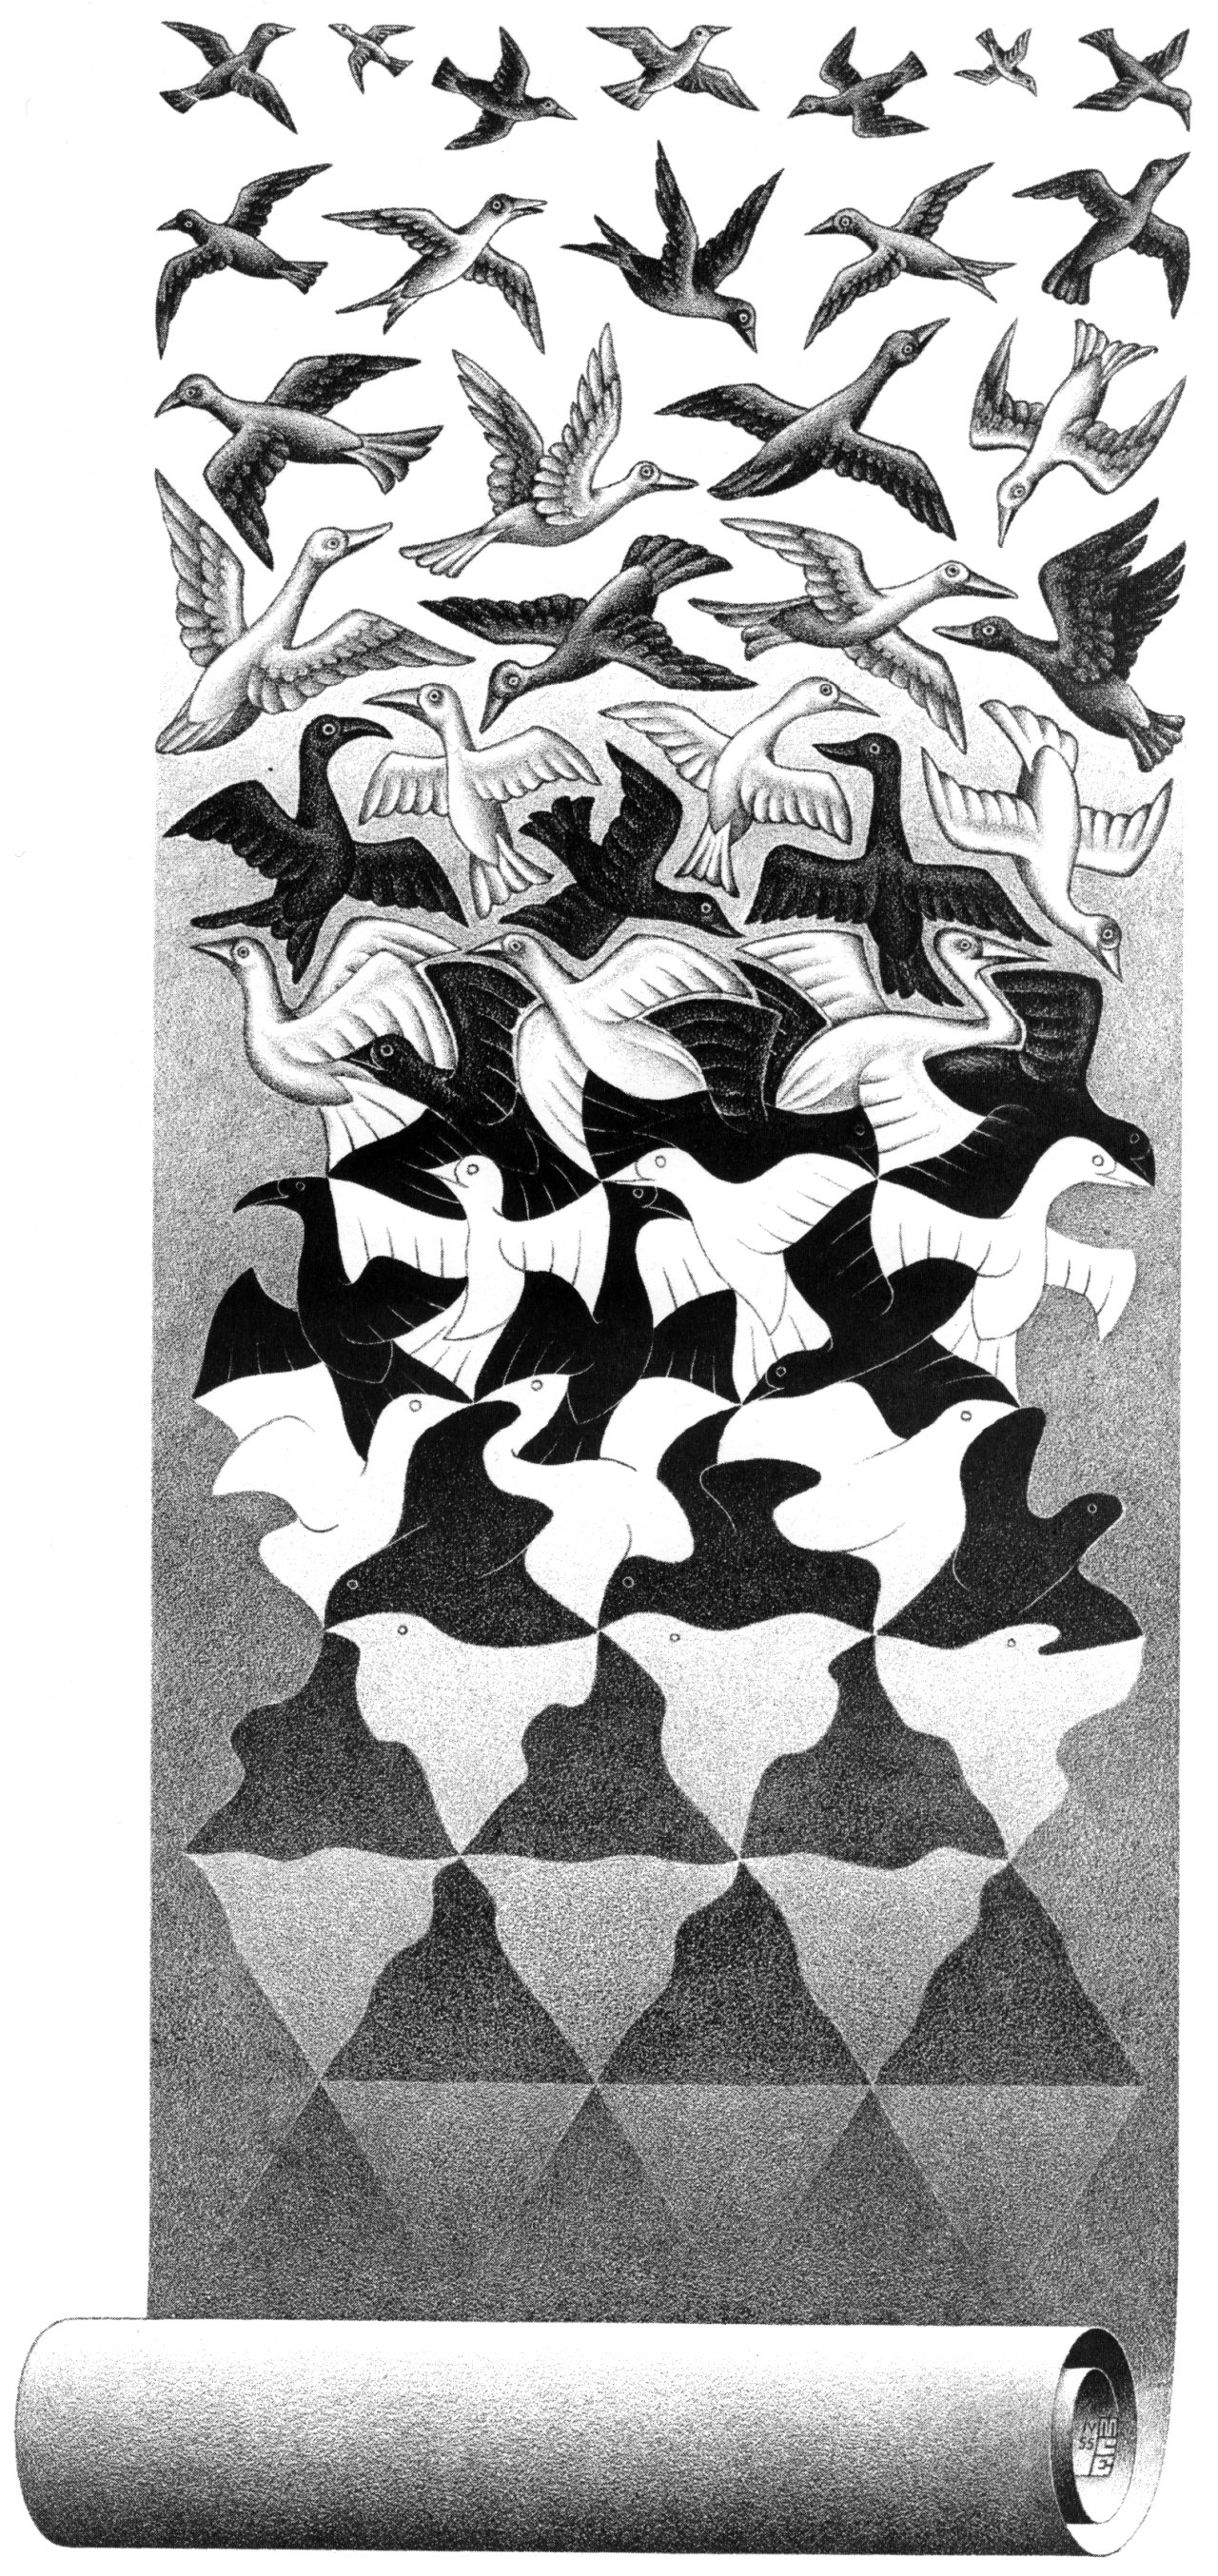
\includegraphics[scale=0.35]{img/Escher-Liberation-1955.eps}
 \captionsetup{labelformat=empty}
 \caption{艾舍尔《解放》}
 \label{fig:Escher-liberation}
\end{wrapfigure}

我们人类在长期的生产生活中逐渐养成了对事物分类整理的习惯。不同但相近的东西被归为一类。对整个类适用的性质和方法,对类中的不同事物都有效。这样我们就从解决具体的单一的问题,提高到一下子解决整类的抽象的问题,极大地丰富了我们认识掌握世界的能力。

在第一章中,我们曾经从自然数的累加和阶乘中归纳抽象出了“叠加”操作。我们观察它们相似的结构,将累加中的0和阶乘中的1抽象成单位元,将累加中的加法和阶乘中的乘法抽象成某种二元运算,这样就在更高的层次抽象出了自然数的叠加。进而可以用这一抽象的叠加操作解决诸如斐波那契数列这样的一大类和自然数同构的问题。

再举一个例子。我们在第一章中,还定义了列表上的抽象叠加操作$foldr$。可以利用这个抽象工具把一列数累加起来:$sum = foldr(0, +)$,也可以把一列数乘到一起:$product = foldr(1, \times)$。在计算机程序中,人们可以定义一种叫做“二叉搜索树”的数据结构。第二章中,我们曾经介绍过二叉树的定义。二叉搜索树是一种特殊的二叉树,它要求树中元素的类型A是可以比较的\footnote{这里比较的含义是抽象的,例如可以比大小,也可以是比较单词在字典中的先后顺序},并且对于任意分支节点,节点左侧子树中的所有元素都在此节点的元素之前,而右子树中的所有元素都在此元素之后。对排序二叉树,我们可以定义一个插入操作:

\[
\begin{array}{rcl}
  insert(nil, x) & = & node(nil, x, nil) \\
  insert(node(l, y, r), x) & = & \left.
  \begin{cases}
  x < y\ : & node(insert(l, x), y, r) \\
  x > y\ : & node(l, y, insert(r, x))
  \end{cases} \right.
\end{array}
\label{eq:BST-insert}
\]

根据这一定义,将一个元素$x$插入到二叉搜索树时,如果树为空,则结果为一个$node(nil, x, nil)$;否则,需要进一步比较$x$和分支节点中的元素$y$,如果$x$在前(用小于号代表),则递归地插入到左子树,否则地归地插入到右子树。联想累加和阶乘,插入操作和它们有什么相似之处呢?插入也是一个二元操作,而nil相当于单位元。这样我们就可以用抽象的叠加操作,将一列数字变成一棵搜索树:

\[
build = foldr(nil, insert)
\]

图\ref{fig:bst-example}展示了计算$build\ [4, 3, 1, 8, 2, 16, 10, 7, 14, 9]$产生的一棵二叉搜索树。

\begin{figure}[htbp]
  \centering
  \includegraphics[scale=0.5]{img/bst-example.ps}
  \caption{通过叠加产生的二叉搜索树}
  \label{fig:bst-example}
\end{figure}

我们人类对加法的认识也经历了类似的过程,最初的加法是针对具体事物的,例如采集的果实或者猎物。然后逐渐将具体事物的意义去除变成了针对抽象整数的加法。后来对数的认识扩充到了分数,虽然分数的具体相加过程和整数大相径庭,需要先对分母进行通分,然后将分子按照整数的法则相加,最后再进行约分。但是我们进一步将这两种不同的操作抽象成了有理数上的加法,人们深入思考它们的本质和性质,在每一次扩充数的认识时,都重新定义更加抽象的加法。从而有了实数上,复数上的加法。人们发现,对去除了具体意义的抽象事物成立的方法具备更大的应用范围。抽象方法能解决一类问题,而不是单一问题。计算机编程中逐渐发展出的面向对象方法,带泛型的类型系统,和动态类型系统都是某种意义上对抽象的一种支持机制。

在发展抽象的方法和工具时,必须时刻关注一个问题:“某一种抽象的适用范围有多大?什么情况下这一抽象会失效?”如果忽略了这一点,就会产生令人啼笑皆非的结果。比如人们总结抽象出了无穷几何级数的累加公式:$1 + x + x^2 + x^3 + ... = 1/(1-x)$。并用它成功解决了芝诺悖论\footnote{古希腊哲学家芝诺提出了四个著名的悖论,这里是指阿基里斯与乌龟悖论。阿基里斯是古希腊著名的英雄。芝诺假设阿基里斯追赶前面的乌龟,当他跑到乌龟出发的位置时,乌龟已经向前移动了一小段距离。阿基里斯必须继续跑到乌龟的新位置,但是此时乌龟又向前移动了。重复这一过程,芝诺认为阿基里斯永远赶不上乌龟。本书在第六章详细解释芝诺悖论。}。但是17世纪的数学家们把-1代入这个公式得到了$1 - 1 + 1 - 1 + ... = 1/2$这样的结果。这时有人提出了不同的意见:$S = (1 - 1) + (1 - 1)+ ... = 0$;还有人认为:$S = 1 + (-1 + 1) + (-1 + 1) + ... = 1$。有人赞同1/2的结果,因为$S = 1 - (1 - 1 + 1 - 1 + ...) = 1 -S$,解方程得$S = 1/2$。意大利数学教授格兰迪(1671 - 1742)还发现了更令人吃惊的结论。通过无穷级数:

\[
\begin{array}{l}
\dfrac{1}{1 + x + x^2} = 1 - x + x^3 - x^4 + x^6 - x^7 + ... \\[2ex]
\dfrac{1}{1 + x + x^2 + x^3} = 1 - x + x^4 - x^5 + x^8 - x^9 + ... \\
...
\end{array}
\]

令$x = 1$,可以得到无穷级数$1 - 1 + 1 - 1 + 1 - 1 + ...$的和可以等于1/3, 1/4, ...就连大数学家莱布尼茨也主张,它的和可能是0或者1,而且概率相等,所以其“真”值应该是它们的平均值1/2。格兰迪还做出了另一个“奇妙”的解释:父亲留给两个儿子一块宝石,由兄弟二人轮流保存,每人一年。于是,交给对方保存的时候,可以说所有权是0,自己保存的时候,可以说所有权是1,而平均而言,每人的所有权为1/2\cite{HanXueTao16}。这些奇怪的问题,要等到法国数学家柯西引入无穷级数收敛性后才得以解决。

编程中也有类似的问题。有一次在编写“自然归并排序”的算法时\footnote{自然归并排序是一种把一组元素按照大小顺序排列好的方法。它首先将元素分成若干组,每组中的元素顺序已经排好了。然后不断将这些组合并直到最后全部排好序。详细可参考\cite{LiuXinyu2017},第368页。},我需要将一列元素分成从大到小的若干组,例如把序列\texttt{[15, 9, 0, 12, 11, 7, 10, 5, 6, 13, 1, 4, 8, 3, 14, 2]}分组成\texttt{[[15, 9, 0], [12, 11, 7], [10, 5], [6], [13, 1], [4], [8, 3], [14, 2]]}。我知道标准库中提供了一个抽象工具\texttt{groupBy},它可以根据一个定义好的条件完成分组,例如:\texttt{groupBy (==) "Mississippi"}会得到结果\texttt{["M", "i", "ss", "i", "ss", "i", "pp", "i"]}。这样连续相等的元素就被分在一组。然而当我把大于等于作为分组条件,却得到了一个不正确的结果。\texttt{groupBy (>=) [15, 9, 0, 12, 11, 7, 10, 5, 6, 13, 1, 4, 8, 3, 14, 2]}产生的结果是\texttt{[[15, 9, 0, 12, 11, 7, 10, 5, 6, 13, 1, 4, 8, 3, 14, 2]]}。经过分析,原来\texttt{groupBy}是通过\texttt{span}实现的:

\lstset{language=Haskell, frame=single}
\begin{lstlisting}
groupBy _  []      = []
groupBy eq (x:xs)  = (x:ys) : groupBy eq zs
    where (ys, zs) = span (eq x) xs

span _ []        = ([], [])
span p xs@(x:xs')
     | p x       = let (ys, zs) = span p xs' in (x:ys, zs)
     | otherwise = ([], xs)
\end{lstlisting}

这样\texttt{span}就会连续判断15是否大于等于下一个元素,由于15恰好是整个列表中最大的,所以全部被归为了一组。实际上\texttt{groupBy}接受的分组条件是一个“抽象的相等”,它必须满足三个性质:自反性、对称性、和传递性:

\begin{itemize}
\item 自反性。$x = x$,即任何元素和它自己相等;
\item 对称性。若$x = y$,则$y = x$,即比较的顺序不影响结果。
\item 传递性。若$x = y$并且$y = z$,则$x = z$,如果两个元素相等,并且其中的一个和第三个元素相等,则这三个元素相等;
\end{itemize}

当对列表“Mississippi”使用等号作为条件分组时,三个条件都被满足,产生了正确的结果。但当将大于等于号($\geq$)作为“相等”条件传入时,就违反了自反性和对称性。这就是得到错误结果的原因。

本章我们介绍一些抽象的代数结构,它们不仅仅是对数的抽象,而且是对事物的概念、性质和关系的抽象。是很多伟大的思想和心智的结晶。

\section{群}

\begin{wrapfigure}{R}{0.4\textwidth}
 \centering
 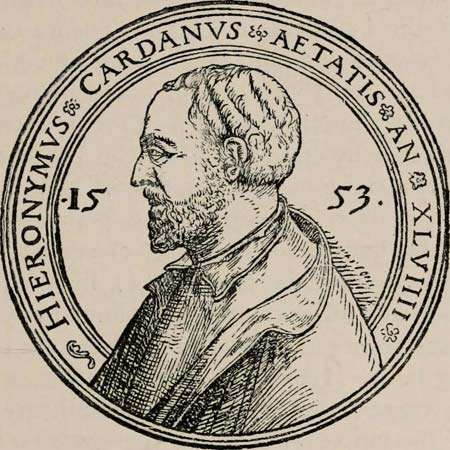
\includegraphics[scale=0.3]{img/Cardano.eps}
 \captionsetup{labelformat=empty}
 \caption{卡尔丹(Gerolamo Cardano, 1501-1576)}
 \label{fig:Cardano}
\end{wrapfigure}

提到群论(Group theory),就不得不提人类解方程的历史。方程是我们祖先发展出的一个强大工具。人们从古埃及的纸草书和古巴比伦的泥板书中发现,这些古代文明已经掌握了一元一次和二次方程的解法。但是一般三次方程的解法却一直没有进展。到了16世纪,经过意大利数学家们的努力,终于得到了一般三次方程和四次方程的根式解。最终卡尔丹在他的著作《大术》中总结人类历史上这千余年的结果。这些进展并不仅仅是未知数次数的提升,我们对数还有了全新的认识。早期二次方程的负根都被舍弃了,人们认为负数没有意义。不仅如此,人们认为方程的系数也必须是正数,在我们今天看来普通的方程$x^2 - 7x + 8 = 0$,必须用$x^2 + 8 = 7x$的形式来处理。在《大术》中,卡尔丹列出了20种不同类型的四次方程,他说还有67种其它类型的四次方程没有给出,原因仅仅是因为四次方程各项的系数可以为负数和零\cite{HanXueTao2012}。直到法国数学家韦达才将方程的形式统一。在解方程时,负数的根式一直被认为是无意义的。但是卡尔丹在解三次方程,例如$x^3 = 15x +4$时,他的公式给出了$\sqrt[3]{2 + \sqrt{-121}} + \sqrt[3]{2 - \sqrt{-121}}$这样的中间结果。而我们知道这一方程有三个实根4, $-2 \pm \sqrt{3}$。这些问题拓展了我们对虚数的认识,并最终在高斯的手中,建立了代数基本定理\footnote{高斯一生多次证明了代数基本定理。1799年,22岁的高斯在其博士论文中证明了实系数一元$n$次方程至少有一个复数根。由此推出$n$次方程有且仅有$n$个复根(重根按重数计算)。高斯又在1815和1816年给出了另外两个证明。1849年,在庆祝取得博士学位50周年的纪念会上,高斯又发表了第四个证明,并把系数也推广到了复数。}。

\begin{figure}[htbp]
%\begin{wrapfigure}{R}{0.3\textwidth}
 \centering
 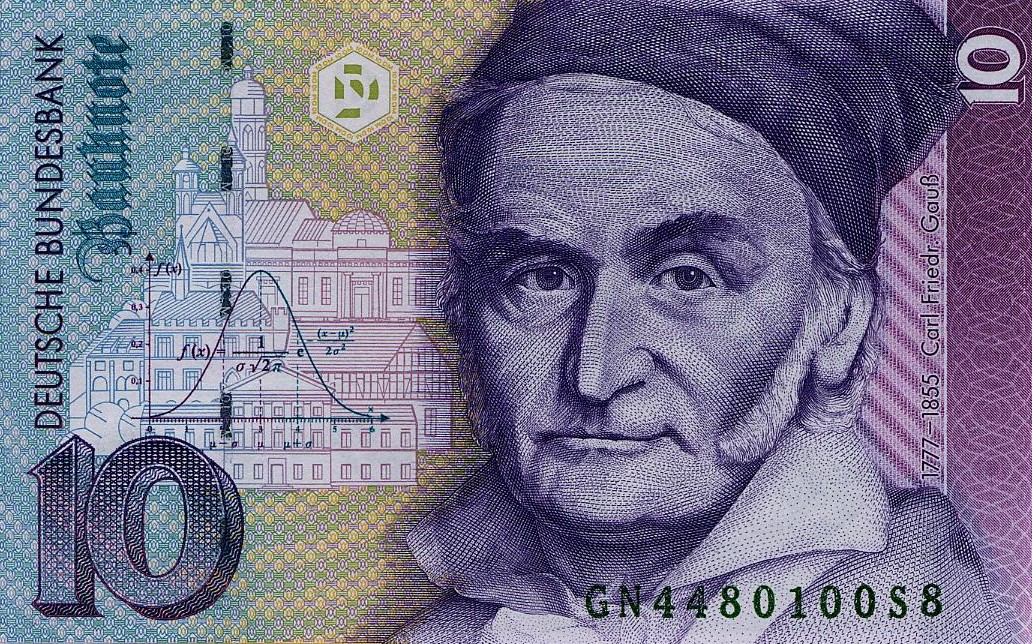
\includegraphics[scale=0.25]{img/Gaus.eps}
 \captionsetup{labelformat=empty}
 \caption{十马克上的高斯像。高斯(1777-1855)}
 \label{fig:Gaus}
%\end{wrapfigure}
\end{figure}

然而接下来在寻找五次及以上方程的根式解时,人们遇到了前所未有的困难。经历了200多年的苦苦寻找,终于在19世纪迎来了出乎意料的结果。法国的天才少年伽罗瓦利用他创建的群论,彻底解决了这个问题。

%\begin{figure}[htbp]
\begin{wrapfigure}{L}{0.4\textwidth}
 \centering
 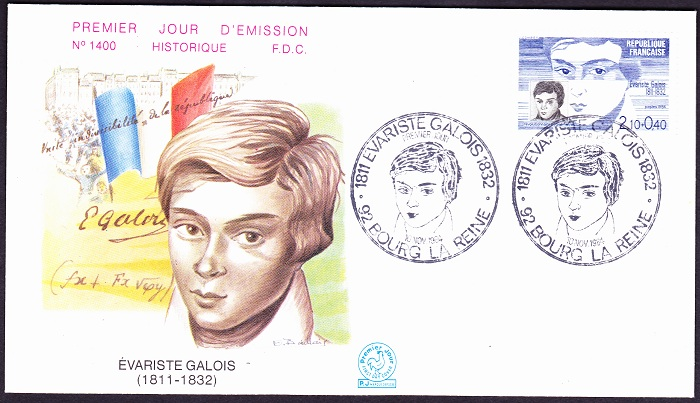
\includegraphics[scale=0.4]{img/galois.eps}
 \captionsetup{labelformat=empty}
 \caption{伽罗瓦(1811 - 1832)}
 \label{fig:Galois}
\end{wrapfigure}
%\end{figure}

伽罗瓦短短的20年人生上演了一幕悲剧,然而他身后却开辟了抽象代数这一数学分支。1811年10月25日,伽罗瓦生于巴黎。他的母亲精通拉丁文和古典文学。在12岁前他一直由母亲进行启蒙教育。1823年,伽罗瓦进入巴黎的一所久负盛名的中学读书。到了14岁,他开始如饥似渴地学习起数学来。他找来一本勒让德改编的《几何原本》,像读小说一样迅速地掌握了。15岁时,他已经四处寻找拉格朗日的原著来读了。他的水平迅速超出了老师的能力范围。16岁时,他开始尝试解五次方程,经历了失败后他开始反思五次方程是否有根式解。但是这位天才少年除了数学对其他学科都不感兴趣。这让他的老师头疼不已。

1828年6月,伽罗瓦参加了法国最富盛名的巴黎综合工科学校的入学考试。在数学口试中,他认为某些结论很显然,于是不进行解释,结果“在某个领域的知识太多,而在其他领域的知识太少”的伽罗瓦落榜了。他只好回到学校继续读书。

1829年4月,伽罗瓦发表了第一篇关于连分数的论文。在这一时期,伽罗瓦在多项式方程上取得了重大的发现。他向法国科学院提交了两篇论文。但由于种种原因,论文没有通过\footnote{有说法认为由于审稿人柯西的疏忽这些论文丢失了。柯西实际上推荐了伽罗瓦的论文,但认为不够清晰,不能发表。人们普遍认为柯西认识到了伽罗瓦工作的重要性, 他只是建议将这两篇论文合并成一个, 以便能够角逐科学院的数学大奖。柯西是当时著名的数学家, 虽然与伽罗瓦的政治观点不同, 但仍认为伽罗瓦能够赢得大奖。\cite{Wiki-Galois}}。打击接踵而至,1829年7月28日,伽罗瓦的镇长父亲因屈服于政敌的恶意攻击自杀身亡\footnote{他与村里的牧师发生了激烈的政治争执后自杀\cite{Wiki-Galois}。}。8月3日,伽罗瓦在服丧期间第二次也是最后一次参加他渴望的巴黎综合工科学校的入学考试。父亲的去世多少对他有影响。在口试阶段,主考官问他一个对数级数的结果是怎样得来的。伽罗瓦跳过了中间步骤说结果很显然,这令考官很恼火,结果他又没有通过。据说伽罗瓦愤怒地把黑板擦投到了主考官的脸上。最后他不得不参加高等师范学校的考试。当时的数学主考官写道:“该生在表达自己的想法时有时很晦涩, 但他很聪明, 表现出非凡的研究精神。”

1830年,在柯西的建议下,伽罗瓦把论文提交给了科学院秘书傅里叶以角逐法兰西科学院的数学大奖。傅里叶把论文带回家中,但未及审阅就去世了。结果伽罗瓦的论文丢失,科学院于1830年6月把大奖授予了阿贝尔\footnote{年轻的阿贝尔已于1829年4月6日在贫病交加中去世了,年仅27岁。他是椭圆函数领域的开拓者,阿贝尔函数的发现者。第一个证明了五次方程无根式解。他还研究了更广的一类代数方程,后人发现这是具有交换的伽罗瓦群的方程。为了纪念他,后人称交换群为阿贝尔群。}和雅可比\cite{HanXueTao2009}。

伽罗瓦生活在政治动荡时期。1830年法国爆发了七月革命\footnote{拿破仑在滑铁卢惨败后,波旁王朝复辟。查理十世清洗了军队中曾为拿破仑效力的军人,引起了人民的不满。并在政治经济、文化宗教和外交中不断失政。查理十世在7月25日颁布圣卢克法令,宣布限制出版自由,解散议会,修改选举法。直接引发了人民的武装起义,通过革命推翻波旁王朝,拥戴路易$\cdot$菲利普登上王位,建立七月王朝。}。因为激进的革命立场,伽罗瓦被学校开除了。他参加了国民自卫军,一边革命一边进行数学研究。1830年12月,国民自卫军被解散,伽罗瓦曾经一度被捕, 但于1831年6月15日被判无罪释放。1831年7月14日法国国庆,伽罗瓦穿上了被解散的国民自卫军军装,拿着上膛的长短枪支上街游行。他因此再次被判入狱6个月。在此之前的1831年1月17日,在数学家泊松的建议下,伽罗瓦又一次将他的方程理论提交给法国科学院。结果泊松也没有能理解伽罗瓦的全新思想。7月4日,负责论文审阅的泊松声称:“论证既不够清晰,又不够详尽,使我们无法判断其严格性\footnote{但是,泊松在论文审阅的报告结尾处鼓励道:“我们建议作者应公布他的全部工作, 以便形成一个明确的意见。”}。”由于伽罗瓦在7月14日被捕,直到10月份他在狱中才收到论文拒绝发表的消息。心高气傲的伽罗瓦反应强烈,他放弃了正规学术途径,转而求助于他的朋友奥古斯特$\cdot$谢瓦利耶(Auguste Chevalier)私人发表论文。伽罗瓦注意到了泊松的建议,他在狱中开始整理数学手稿,并不断完善他的思想,直到1832年4月29日出狱。

出狱后不久,伽罗瓦因为爱情卷入了一场无谓的决斗。5月29日决斗前夕,深信自己将在决斗中死去的伽罗瓦写了三封信。最长的第三封信是写给朋友谢瓦利耶的,短短7页中包含了一份数学思想纲要和三份手稿。这份纲要十分简洁,但内容却极为丰富。只有在后来人把它展开的时候,其重要性才渐渐为人所理解。而且预见了很久以后的发现,证明了伽罗瓦深刻的洞察力。数学家赫尔曼$\cdot$外尔认为:“从创新程度与思想深度来看,这封信有可能是有史以来份量最重的一篇文字。”信中还有一些后人读来无比惋惜的文字:“这些题目并非我已研究的全部……我没有时间,在我有兴趣的领域里,我已宣布但尚未证明,从而使人怀疑的定理确实是太多了。”其中最令人难忘的,也是最悲伤的话语是:“我没有时间了。”在信的末尾,他要求他的朋友“请求雅可比或者高斯就这些定理的重要性(而不是正确与否)公开发表他们的看法。我希望将来有人能意识到它们是有益的。”

1832年5月30日早晨,伽罗瓦在决斗受了重伤,一个路过的农民发现了他。9点半,他被送到医院。他拒绝了牧师的祈祷,对赶来的弟弟说:“阿尔弗莱德,不要哭。在20岁就死去,需要我全部的勇气。”次日上午10时,伽罗瓦停止了呼吸。关于决斗的原因,有各种不同的说法。人们不知道这是一个悲惨的爱情事件还是政治谋杀。无论是哪一种,一位世界上最杰出的数学家在他20岁时被杀死了,他研究数学只有5年,而其全部数学成果仅有67页。

谢瓦利耶和伽罗瓦的弟弟按照他的遗愿将其工作发表在《百科评论》上,但没有对当时的数学发展产生影响。也许是因为它太晦涩简略了。直到14年后的1846年,法国数学家刘维尔领悟到伽罗瓦思想的价值,将这些论文编辑发表在极有影响的《纯粹与应用数学》杂志上。在对论文的介绍中,刘维尔对伽罗瓦的悲剧进行了反思:“过分地追求简结是导致这一缺憾的原因。人们处理像纯粹代数这样抽象和神秘的事物时,应该首先尽力避免这样做。事实上,当你试图引导读着远离习以为常的思路进入较为困惑的领域时,清晰性是绝对必须的……但是现在一切都改变了,伽罗瓦再也回不来了!我们不要再过分地做无用地批评,让我们把缺憾抛开,找一找有价值的东西……我的热心得到了好报,在填补了一些细小的缺陷后,我看出伽罗瓦用来证明这个定理的方法是美妙和完全正确的,在那个瞬间,我体验到了一种强烈的愉悦。”1870年法国数学家约当根据伽罗瓦的思想,撰写了《置换与代数方程》一书,伽罗瓦的最主要成就是提出了“群”的概念,并用群论彻底解决了根式求解代数方程的问题,而由此发展出了一整套关于群和域的理论。为了纪念他,人们称之为伽罗瓦理论。正是这套理论创立了抽象代数学,标志着数学发展现代阶段的开始。有人评论道:“伽罗瓦一心想要参加的是政治革命,然而实际上所引发的却是数学革命。\cite{StepanovRose15}”

\subsection{群的定义}

下面我们来了解一下群的定义。

\begin{definition}群是一个集合$G$与其上定义的某种二元运算$\cdot$。记为$(G, \cdot)$。它们遵循四条公理:
\begin{enumerate}
\item 封闭性公理:对任何$a, b \in G$,运算结果$a \cdot b \in G$;
\item 结合性公理:对任何$a, b, c$,有$(a \cdot b) \cdot c = a \cdot (b \cdot c)$;
\item 单位元公理:$G$中存在一个元素$e$,使得对任何$a \cdot e = e \cdot a = a$;
\item 消去公理:对任何$a \in G$,都存在一个逆元$a^{-1}$使得$a \cdot a^{-1} = a^{-1} \cdot a = e$。
\end{enumerate}
\end{definition}

方便起见,我们有时称二元运算为“乘法”,并且省略掉点,将$a \cdot b$写成$ab$。我们称$e$为单位元。一个群的元素个数可以有限也可以无限,分别称为有限群和无限群。元素的个数叫做这个群的阶。

群的“乘法”运算并不一定像数的乘法运算那样满足交换律。例如所有元素为实数的可逆矩阵与矩阵乘法组成一个群。但矩阵乘法是不可逆的。如果群中的二元运算满足交换律,则称为交换群。为了纪念挪威数学家阿贝尔,人们称交换群为阿贝尔群。

为了帮助理解这一抽象定义,我们来看一些具体的群的例子。

\begin{enumerate}
\item 整数加法群:群元素是全体整数,二元运算是加法。简称为整数加群;
\item 所有整数除以5的余数构成的集合,也就是$\{0, 1, 2, 3, 4\}$。二元运算是相加后再除以5取余数。例如$3 + 4 = 7 \bmod 5 = 2$。这样构成的群称为整数模5加法群,记为$Z_5$。通过取余数对整数进行分类叫做模$n$剩余类;
\item 转动魔方所形成的群:群元素是各种魔方转动的方式\footnote{魔方的旋转方式共有18种。可以沿着正面、反面、顶面、底面、左面、右面旋转,分别用字母$F$、$B$、$T$、$D$、$L$、$R$代表,每面可以旋转90度、180度、-90度。例如左面旋转90度、180度、-90度分别可以记为:$L$、$L^2$、$L'$\cite{Wiki-Rubik-Cube-group}。再加上恒等变换,一共19个元素。},二元运算是先进行某种转动后再进行另一种转动。这种运算常被称作转动的合成;

\begin{figure}[htbp]
%\begin{wrapfigure}{L}{0.4\textwidth}
 \centering
 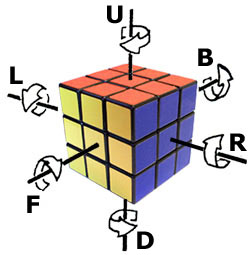
\includegraphics[scale=0.8]{img/Rubik_cube_notation.eps}
 %\captionsetup{labelformat=empty}
 \caption{魔方六个面共有18种转动方式,再加上恒等变换。这些转动方式在合成下构成一个群。}
 \label{fig:Rubik-cube-notation}
%\end{wrapfigure}
\end{figure}

\item 平面绕某点的所有旋转构成一个群。群元素是所有的旋转角度,二元运算是先旋转某一角度,然后再旋转另一角度。
\end{enumerate}

而下面这些不是群:

\begin{enumerate}
\item 所有不等于零的整数和乘法不构成群,我们不能规定单位元为1,这样3没有逆元(1/3不是整数);
\item 同理,模5的余数集合$\{0, 1, 2, 3, 4\}$和模5的乘法不构成一个群,但如果把5的整倍数去掉,则集合$\{1, 2, 3, 4\}$和模5的乘法构成一个群。可以从下面的“乘法表”看出来:

  \begin{tabular}{c|cccc}
    & 1 & 2 & 3 & 4 \\
  \hline
  1 & \textbf{1} & 2 & 3 & 4 \\
  2 & 2 & 4 & \textbf{1} & 3 \\
  3 & 3 & \textbf{1} & 4 & 2 \\
  4 & 4 & 3 & 2 & \textbf{1}
  \end{tabular}

因此,单位元是1,它的逆元是其本身;2和3互为逆元,4的逆元还是4;
\item 虽然模5的非零余数在模乘法下构成一个群,但是模4的非零余数在模乘下却不构成群。观察模4的乘法表:

  \begin{tabular}{c|cccc}
    & 1 & 2 & 3 \\
  \hline
  1 & 1 & 2 & 3 \\
  2 & 2 & \textbf{0} & 2 \\
  3 & 3 & 2 & 1 \\
  \end{tabular}

注意到$(2 \times 2) \bmod 4 = 0$,不在集合$\{1, 2, 3\}$中。这个反例告诉我们,只有和$n$互素的余数集合,在模$n$乘法下才能构成群,这种群称为整数模$n$乘法群。自然,如果$p$是素数,则$\{1, 2, ..., p-1\}$构成模$p$乘法群。
\item 全体有理数在乘法下不构成一个群。尽管任何形如$p/q$的有理数都有逆元$q/p$,但是0没有逆元。所有非零有理数在乘法下才构成一个群。
\end{enumerate}

\begin{Exercise}
\Question{全体偶数在加法下是否构成一个群?}
\Question{能否找到一个整数的子集,使得它在整数乘法下构成一个群?}
\Question{所有正实数在乘法下是否构成一个群?}
\Question{整数在减法下是否构成一个群?}
\Question{举一个只有两个元素的群的例子。}
\Question{魔方群的单位元是什么?$F$的逆元是什么?}
\end{Exercise}

\subsection{幺半群与半群}
群的限制条件比较严格,从上一节的反例中,我们看到有一些常用的代数结构无法满足群的全部条件。有时我们并不需要一定能够取逆元,如果放宽条件,就可以得到幺半群(monoid)这种结构。

\begin{definition}
{\em 幺半群}是一个集合$S$和其上定义的二元运算$\cdot$,它们遵循两条公理:
\begin{enumerate}
\item 结合性公理:$S$中和任何三个元素满足$(a \cdot b) \cdot c = a \cdot (b \cdot c)$;
\item 单位元公理:$S$中存在一个元素$e$,使得对任何$a \cdot e = e \cdot a = e$。
\end{enumerate}
\end{definition}

可以看到幺半群与群的定义类似,只是去掉了取逆运算的消去公理。可以立即看到,上一节群的反例中有不少是幺半群,例如整数乘法构成幺半群,单位元是1。幺半群在编程中很常见。我们在下一章介绍范畴论时还会再仔细讲解幺半群这一特别重要的结构。下面是一些幺半群的例子:

\begin{enumerate}
\item 给定字符集后,长度有限的字符串在拼接操作下构成幺半群。幺半群的元素是字符串,二元运算是拼接操作。单位元是空串。
\item 由字符串推广到列表(List A),在连接操作下构成幺半群。幺半群的元素是列表,二元运算是连接操作($\doubleplus$)。单位元是空列表nil。

为此,我们可以写出以下的程序,用幺半群来定义字符串和列表的代数结构。

\begin{lstlisting}
instance Monoid (List A) where
    e = nil
    (*) = (++)
\end{lstlisting}

这样针对字符串和列表的的“叠加”操作,完全可以将抽象程度提升到幺半群上来\footnote{我们将在下一章讲解范畴论时介绍如何实现这样的抽象叠加操作}。例如下面的“合并”操作定义对任何幺半群都有效:

\[
concat = foldr\ e\ (*)
\]

这样就可以用$concat$合并列表,如

$concat\ [[1], [2], [3], [1, 2], [1, 3], [2, 3], [1, 2, 3], [1, 3, 2]]$的结果是[1, 2, 3, 1, 2, 1, 3, 2, 3, 1, 2, 3, 1, 3, 2]。

\item 堆(heap)是编程中一种常见的数据结构,堆顶元素总是最小的堆称为最小堆(或小顶堆、小根堆)。有一种“斜堆”(skew heap)可以用上一章定义的二叉树来实现(\cite{LiuXinyu2017}第7.3节):

\begin{lstlisting}
data SHeap A = nil | node (SHeap A, A, SHeap A)
\end{lstlisting}

可以看出,除了名称,斜堆的定义和二叉树完全一样。非空堆的最小元素在树的根节点中。定义斜堆的“归并”(merge)运算如下:

\[
\begin{array}{rcl}
merge(nil, h) & = & h \\
merge(h, nil) & = & h \\
merge(h_1, h_2) & = &
  \begin{cases}
  k_1 < k_2 : & node(merge(r_1, h_2), k_1, l_1) \\
  \text{否则}: & node(merge(h_1, r_2), k_2, l_2)
  \end{cases}
\end{array}
\]

如果其中任一堆为空,则归并结果为另一个堆。非空情况下,$h_1$和$h_2$分别可以表示为$node(l_1, k_1, r_1)$和$node(l_2, k_2, r_2)$。我们比较根节点,选择较小的作为新的根。然后把含有较大元素的树合并到某一子树上。最后再把左右子树交换。若$k_1 < k_2$,选择$k_1$作为新的根。我们既可以将$h_2$和$l_1$合并,也可以将$h_2$和$r_1$合并。不失一般性,我们合并到$r_1$上。然后交换左右子树,最后的结果为$(k_1, merge(r_1, h_2), l_1)$。注意这个归并的二元运算是递归的。这样所有斜堆组成的集合,在这一归并运算下构成一个幺半群。单位元是空堆nil。

\item 堆也可以用上一章介绍的多叉树实现。有一种堆叫做配对堆(pairing heap)它的定义如下(\cite{LiuXinyu2017}第9.4节):

\begin{lstlisting}
data PHeap A = nil | node (A, List (PHeap A))
\end{lstlisting}

除了名称外,这个定义和上一章的多叉树的结构完全相同。这是一个递归定义,一个配对堆要么为空,要么是一棵多叉树,包含一个根节点和一组子树。非空堆的最小元素在多叉树的根节点中。我们可以定义配对堆的归并操作:

\be
\begin{array}{rcl}
merge(nil, h) & = & h \\
merge(h, nil) & = & h \\
merge(h_1, h_2) & = &
  \begin{cases}
  k_1 < k_2 : & node(k_1, h_2 : ts_1)) \\
  \text{否则} : & node(k_2, h_1 : ts_2)) \\
  \end{cases}
\end{array}
\ee

如果任一堆为空,则归并结果为另一个堆。非空情况下,两个堆$h_1$和$h_2$分别可以表示为$node(k_1, ts_1)$和$node(k_2, ts_2)$。我们比较两个堆的根节点元素,令根节点较大的一个作为另一个的新子树。这样所有的配对堆组成的集合,在归并操作下构成一个幺半群,单位元是空堆nil。

\end{enumerate}

如果再进一步把单位元的限制也去掉,我们就得到了半群(semigroup)这种代数结构。

\begin{definition}
半群是一个集合和定义在其上的可结合的二元运算。
\end{definition}

半群的二元运算是可结合的,所以满足结合律:半群中的任何三个元素$a$、$b$、$c$满足$(ab)c = a(bc)$。半群的条件更为宽松,下面是一些半群的例子:

\begin{enumerate}
\item 全体正整数构成的加法半群、乘法半群;
\item 全体偶数构成的加法半群、乘法半群。
\end{enumerate}

如前所述,人们常将定义在群、幺半群、半群上的二元运算叫做“乘法”,因此我们可以用“乘方”来表示连续的二元运算。如:$x \cdot x \cdot x = x^3$。一般地,群和幺半群的“幂”可以递归地定义如下:

\[
x^n = \left .
  \begin{cases}
  n = 0 : & e \\
  \text{其它}: & x \cdot x^{n-1}
  \end{cases}
\right .
\]

但是半群没有单位元,所以$n$必须是非零正整数:

\[
x^n = \left .
  \begin{cases}
  n = 1 : & x \\
  \text{其它}: & x \cdot x^{n-1}
  \end{cases}
\right .
\]

\begin{Exercise}
\Question{布尔值构成的集合\{True, False\},在“逻辑或”运算$\lor$下构成一个幺半群。称为任意(Any)逻辑幺半群。它的单位元是什么?}
\Question{布尔值构成的集合\{True, False\},在“逻辑与”运算$\land$下构成一个幺半群。称为全部(All)逻辑幺半群。它的单位元是什么?}
\Question{对可比类型的元素进行比较时,会有三种结果,我们把它们抽象为$\{<, =, >\}$\footnote{一些编程语言,如C、C++、Java用负数、零、正数表示这三种关系。Haskell中用GT, EQ, LE表示。},针对这个集合,定义一个二元运算使得它们构成一个幺半群。这个幺半群的单位元是什么?}
\Question{证明群、幺半群、半群的幂满足交换律:$x^mx^n = x^nx^m$}
\end{Exercise}

\subsection{群的性质}

抽象代数最强大的思想在于我们可以不关心抽象概念所代表的实际物体的含义,而研究抽象结构间内在的规律。这些规律对所有被抽象的物体都适用。如果我们了解了一般群的内在规律,而群元素代表几何的点、线、面,则我们就获得了几何的规律;如果群元素是魔方的旋转,我们就获得了魔方变换的规律;如果群元素是编程中的某种数据结构,我们就得到了这种数据结构上的算法。我们这一节介绍一些群上的重要性质。

\begin{theorem}
群的单位元是唯一的。
\end{theorem}

\begin{proof}
假设存在另一单位元$e'$,使得对任意元素$a$满足$e'a = ae' = a$。我们有$e = ee'= e'$。这样就证明了单位元的唯一性。
\end{proof}

不仅群的单位元是唯一存在的,而且每个元素的逆也是唯一存在的。我们有下面的定理。

\begin{theorem}
逆元唯一存在。对群中的任意元素$a$,都存在且仅存在一个$a^{-1}$使得$aa^{-1} = a^{-1}a = e$。我们称$a^{-1}$为$a$的逆元。
\end{theorem}

\begin{proof}
根据群的消去公理,我们知道逆元存在。所以我们只需要证明逆元唯一。假设存在另一元素$b$,也满足$ab = ba = e$,我们在等式右侧“乘以”$a^{-1}$得:
\[
\begin{array}{rll}
aba^{-1} & = baa^{-1} = ea^{-1} & \\
& \Rightarrow be = a^{-1} & \text{对第二项用结合律} \\
& \Rightarrow b = a^{-1} & \text{逆元唯一}
\end{array}
\]
\end{proof}

\begin{figure}[htbp]
%\begin{wrapfigure}{L}{0.4\textwidth}
 \centering
 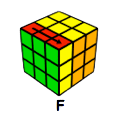
\includegraphics[scale=1.0]{img/Rubik-cube-F.eps}
 %\captionsetup{labelformat=empty}
 \caption{魔方的F变换,连续转动4次回到原位。}
 \label{fig:Rubik-cube-F}
%\end{wrapfigure}
\end{figure}

我们在前面定义了群的阶,群的元素也可以定义阶。对群中的一个元$a$,能够满足$a^m = e$的最小正整数$m$叫做$a$的阶。如果这样的$m$不存在,我们说$a$的阶是无限的。例如前面例子中魔方旋转群中,$F$旋转4次就回到了原位,所以$F$的阶是4,而$F'$旋转两次回到原位,所以它的阶是2。再比如整数模5的乘法群,除了1以外,其他元素的4次幂都模5余1,所以他们的阶都是4。我们有如下有趣的定理。

\begin{theorem}
有限群的每个元素都有有限的阶。
\end{theorem}

\begin{proof}
如果有限群$G$的阶是$n$,对任意元素$a$,构造集合$\{a, a^2, ..., a^{n+1}\}$。这个集合有$n+1$个元,但是群的阶是$n$,所以根据鸽笼原理,一定有两个元素是相等的, 不妨记这两个元素为$a^i$和$a^j$,其中$0 < i < j \leq n + 1$。我们有:
\[
\begin{array}{rcll}
a^ja^{-i} & = & a^{-i}a{i} & \text{由} a^i = a^j \\
a^ja^{-i} & = & e & \text{$a^i$和$a^{-i}$互为逆元} \\
a^{j-i} & = & e & a\text{的阶为} j - i
\end{array}
\]
所以$a$的阶为$j-i$是有限的。
\end{proof}

在第一章,我们比较随意地使用了“同构”一词来形容具有相同内在结构的事物。现在我们可以给出同态和同构的概念了。假设存在从某个集合$A$到另一个集合$B$的映射$f$。$a$和$b$是$A$中的两个元,$f(a)$和$f(b)$是它们在$B$中的像。我们考虑$A$上的二元封闭运算产生的元$a \cdot b$,在映射下在$B$中的像$f(a \cdot b)$。如果对$B$上的二元封闭运算总有

\[
f(a) \cdot f(b) = f(a \cdot b)
\]

\begin{figure}[htbp]
\centering
\begin{tikzpicture}[scale=0.8]
\draw (0, 0) circle[x radius=1cm, y radius=3cm]
      (5, 0) circle[x radius=1cm, y radius=3cm];
\path (0, 3) node[above] {$A$:自然数乘法半群}
      (5, 3) node[above] {$B$:平方数乘法半群};
\path (0, 0) node (b) {}
      (5, 0) node (fb) {}
      (0, 1.5) node (a) {}
      (5, 1.5) node (fa) {}
      (0, -1.5) node (c) {}
      (5, -1.5) node (fc) {};
\filldraw (0, 0) circle (1pt) node[above] {$b$}
      (5, 0) circle (1pt) node[above] {$f(b)$}
      (0, 1.5) circle (1pt) node[above] {$a$}
      (5, 1.5) circle (1pt) node[above] {$f(a)$}
      (0, -1.5) circle (1pt) node[above] {$ab$}
      (5, -1.5) circle (1pt) node[above] {$f(ab)$};
\draw[dashed, ->] (b) to node [above] {$f: x \to x^2$} (fb)
      (a) to [bend left] (fa)
      (c) to [bend right] (fc);
\end{tikzpicture}
\[
\begin{array}{rl}
a = 2 & f(a) = 4 \\
b = 3 & f(b) = 9 \\
ab = 6 & f(ab) = f(a)f(b) = 36
\end{array}
\]
\caption{同构}
\label{fig:isomorphism}
\end{figure}

我们就说$f$是从$A$到$B$的{\em 同态映射}(homomorphism)。如果$f$是满射(surjection,即$B$中所有元素都在$A$中有原像),则称为同态满射。举一个例子,考虑一个奇偶判定函数$odd: Z \to Bool$,它接受一个整数,如果是奇数就返回真值True,否额返回假False。整数在加法下构成一个群。而布尔集合$\{True, False\}$在逻辑或运算下也构成一个群。我们可以很容易验证:

\begin{enumerate}
\item $a$和$b$都是奇数,$odd(a)$和$odd(b)$都为真。它们的和也是奇数,$odd(a+b)$也为真。满足$odd(a) \lor odd(b) = odd(a+b)$;
\item $a$和$b$都是偶数,$odd(a)$和$odd(b)$都为假。它们的和也是偶数,$odd(a+b)$也为假。满足$odd(a) \lor odd(b) = odd(a+b)$;
\item $a$和$b$一奇一偶,$odd(a)$和$odd(b)$一真一假。它们的和为奇数,$odd(a+b)$为真。满足$odd(a) \lor odd(b) = odd(a+b)$;
\end{enumerate}

如果$f$不仅是满射,还是单射(injection)。那么它就是一一映射。这种情况下,我们称$f$是从$A$到$B$的同构映射,简称{\em 同构}(isomorphism)。记为$A \cong B$。同构是一种非常强大的关系,不仅两个群可以同构,半群、幺半群以及其他代数结构也可以同构,如图\ref{fig:isomorphism}所示。如果$A$和$B$同构,那么抽象地来看,它们没有什么区别,只有命名上的不同。如果$A$上有一个代数性质,那么在$B$上也有一个完全类似的性质\cite{ZhangHeRui1978}。另外,$A$与$A$之间的同构映射称为$A$的{\em 自同构}(automorphism)。例如整数加群在取相反数下成为自同构。

\begin{figure}[htbp]
\centering
\begin{tikzpicture}
\path (0, 0) node[below] {猫}
      (0, 2) node[above] {羊}
      (-2, 2) node[above] {狗}
      (-2, 0) node[below] {牛};
\filldraw (0, 0) circle (4pt) node (cat) {} --
   (0, 2) circle (4pt) node (sheep) {} --
   (-2, 2) circle (4pt) node (dog) {} --
   (-2, 0) circle (4pt) node (cow) {};
\draw (dog) -- (cat) -- (cow);

\filldraw[fill=gray, draw=black, pattern=north west lines]
    (3, 0) circle (4pt) node (collar) {} --
    (5.6, 0) circle (4pt) node (bell) {} --
    (4.3, 2.3) circle (4pt) node (milk) {} -- (collar) --
    (4.3, 1) circle (4pt) node (wool) {} -- (bell);
\path (3, 0) node[below] {项圈}
      (5.6, 0) node[below] {铃铛}
      (4.3, 2.3) node[above] {奶}
      (4.3, 1) node[below] {毛};

\draw[dashed, ->] (dog) .. controls (-2.5, 1.5) .. (collar)
    (sheep) to[bend left] (wool)
    (cat) to[bend right] (bell)
    (cow) .. controls (-3, 3) ..(milk);
\end{tikzpicture}
\[
\begin{array}{rl}
f(狗) = 项圈 & f(猫) = 铃铛 \\
f(羊) = 毛 & f(牛) = 奶
\end{array}
\]
\caption{图的同构(graph isomorphsim)具有不同的定义。它反映了看似不同的两个图,具有相同的结构。}
\label{fig:graph-isomorphism}
\end{figure}

面对群这种抽象的代数结构时,具体的例子可以帮助我们理解。我们会不自觉地选出一个自己熟悉的代表,例如整数加群,然后看看各种概念,性质在其上是怎样的。但有时这容易形成一种错觉。感觉群的元素大多是一些实体,例如各种数;并且二元运算大多像普通加法、乘法那样可以交换。我们接下来介绍的“变换群”是一个例外,一方面,它不是阿贝尔群,运算不可交换;另一方面群元素不是数,而是变换。

所谓变换,就是一个集合$A$到$A$自身的映射。记为$\tau : A \to A$。它把集合$A$的元素$a$映射为$\tau(a)$,即$a \to \tau(a)$。一个集合可以有多个不同的变换,例如下面是布尔集合的全部变换,我们记真为$T$、假为$F$。

\[
\begin{array}{rll}
\tau_1 : & T \to T, & F \to T \\
\tau_2 : & T \to F, & F \to F \\
\tau_3 : & T \to T, & F \to F \\
\tau_4 : & T \to F, & F \to T
\end{array}
\]

其中变换$\tau_3$和$\tau_4$是一一变换。针对一个集合$A$,我们将它的全体变换放到一起构成一个新的集合:

\[
S = \{\tau, \lambda, \mu, ...\}
\]

现在我们要规定一个S的二元代数运算,把它叫做乘法。为了方便起见,我们将$\tau(a)$用另一个符号表达:

\[
\tau: a \to a^\tau = \tau(a)
\]

这里$a^\tau$不是$a$的$\tau$次方的意思,它只是一个符号记法,表示变换的意思。我们观察$S$的两个元$\tau$和$\lambda$,

\[
\tau: a \to a^\tau,  \lambda: a \to a^\lambda
\]

那么$a \to (a^\tau)^\lambda = \lambda(\tau(a))$显然也是$A$的一个变换,现在我们规定把这个变换叫做$\tau$和$\lambda$的乘积。

\[
\tau\lambda: a \to (a^\tau)^\lambda = a^{\tau\lambda}
\]

读着不妨从前面布尔变换的集合里取几个变换来计算它们的乘积,不难验证这一乘法适合结合律,因为:

\[
\begin{array}{rl}
\tau(\lambda\mu): & a \to (a^\tau)^{\lambda\mu} = ((a^\tau)^\lambda)^\mu \\
(\tau\lambda)\mu: & a \to (a^{\tau\lambda})^\mu = ((a^\tau)^\lambda)^\mu
\end{array}
\]

现在不难看出当初我们选择乘方符号来表达变换的好处了。选择一套强大的符号系统是多年来数学发展传统和法宝。欧拉、莱布尼茨都是选择和使用符号的大师。对这个乘法来说,$S$的单位元就是$A$的恒等变换$\epsilon: a \to a$。不难验证:

\[
\begin{array}{rl}
\epsilon\tau: & a \to (a^\epsilon)^\tau = a^\tau \\
\tau\epsilon: & a \to (a^\tau)^\epsilon = a^\tau
\end{array}
\]

所以$\epsilon\tau = \tau\epsilon = \tau$。这样$S$对这个乘法来说差不多已经构成一个群了。可惜,虽然说是差不多,到底还是差一点。因为任意变换$\tau$不一定有逆元。例如布尔变换集合中的$\tau_1$,它把任何布尔值都变换成真,不管用这4个变换中的哪一个,都无法把$\tau_1$变换回去。所以$\tau_1$没有逆元。

虽然$S$无法构成群,但是峰回路转,是它的一个子集$G$却有可能构成群。事实上,如果$G$只包含$A$的一一变换,则它在这个乘法下构成群。

我们称,一个集合$A$的若干个一一变换对于上述规定的乘法所作成的群叫做$A$的一个{\em 变换群}(transform group)。并且我们有以下重要的定理:

\begin{theorem}
一个集合$A$的所有一一变换构成一个变换群$G$。
\end{theorem}

变换群一般不是交换群(阿贝尔群),我们可以很容易地找到反例。考虑$\tau_1$是平面上的平移,它把原点(0, 0)移动到(1, 0),变换$\tau_2$是绕原点旋转$\pi/2$,但是:

\[
\begin{array}{rl}
\tau_1\tau_2: & (0, 0) \to (0, 1) \\
\tau_2\tau_1: & (0, 0) \to (1, 0)
\end{array}
\]

\begin{figure}[htbp]
\centering
\begin{tikzpicture}[scale=1]
\draw[->] (-0.5, 0) -- (2, 0) node[right] (x axis) {$x$};
\draw[->] (0, -1.5) -- (0, 1.5) node[above] (y axis) {$y$};
\path (0, -1) node[left] {$a$}
      (1, -1) node[right] {$b$}
      (1, 1) node[above] {$c$};
\filldraw (0, -1) circle(1pt) node (a) {}
          (1, -1) circle(1pt) node (b) {}
          (1, 1) circle(1pt) node (c) {};
\draw[dashed, ->] (a) -- (b);
\draw[dashed, ->] (b) .. controls (1.4, 0) .. (c);
\draw (0, 0) -- (1.2, -1.2)
      (0, 0) -- (1.2, 1.2)
      (1, 0) arc (0:45:1)
      (1, 0) arc (0:-45:1);

\draw[->] (3.5, 0) -- (6.5, 0) node[right] (x axisr) {$x$};
\draw[->] (4, -1.5) -- (4, 1.5) node[above] (y axisr) {$y$};
\filldraw (4, -1) circle (1pt) node[left] (a1) {$a$}
      (5, 0) circle (1pt) node[above] (b1) {$b'$}
      (6, 0) circle (1pt) node[above] (c1) {$c'$};
\draw[dashed, ->] (a1) .. controls (4.7, -0.7) .. (b1);
\draw[dashed, ->] (b1) -- (c1);
\draw (5, 0) arc (0:-90:0.8);
\end{tikzpicture}
\caption{变换顺序不同,结果也不同的例子}
\label{fig:transform-not-abelian}
\end{figure}

因此这一变换群不是阿贝尔群。变换群应用极广,十分重要,我们有一个很强的结论:

\begin{theorem}
任何一个群都同一个变换群同构。
\end{theorem}

% TODO:附录
我们把以上两个定理的证明放在附录以供参考。这个定理告诉我们,任意一个抽象的群都能在变换群里找到一个具体的实例。换一句话说,我们不必害怕,将来会找到一个抽象群,这个群完全是我们脑子里造出来的空中楼阁\cite{ZhangHeRui1978}。

\begin{Exercise}
\Question{奇偶判断函数在整数加群$(Z,+)$和布尔逻辑与群$(Bool, \land)$下是否构成同态?去除0元素的整数乘法群呢?}
\Question{假定两个群$G$和$G'$在映射下同态,群$G$中的元$a \to a'$,那么$a$和$a'$的阶是否相同?}
\Question{证明一个变换群的单位元一定是恒等变换。}
\end{Exercise}

\subsection{置换群}

我们现在介绍伽罗瓦用来判定方程是不是有根式解的群——置换群。这种群是变换群的一种特例。我们首先定义置换的概念。一个有限集合的一一变换叫做一个{\em 置换}。一个有限集合的若干个置换作成的一个群叫做一个{\em 置换群}(permutation group)。进一步,一个包含$n$个元素的集合的全体置换作成的群叫做$n$次{\em 对称群}(symmetric group)。这个群用$S_n$来表示。

由高中的排列组合我们知道,$n$元的置换一共有$n!$个。所以$n$次对称群$S_n$的的阶是$n!$。一个置换把集合的元$a_i$映射为$a_{k_i}$,其中$i = 1, 2, ..., n$。所以这一置换完全可以由$(1, k_1), (2, k_2), ..., (n, k_n)$这$n$对数来确定。我们可以把这一置换写成:

\[
\begin{pmatrix}
1 & 2 & ... & n \\
k_1 & k_2 & ... & k_n
\end{pmatrix}
\]

例如

\[
\begin{pmatrix}
1 & 2 & 3 & 4 & 5 \\
2 & 5 & 4 & 3 & 1
\end{pmatrix}
\]

就表示了一个置换。明显这样第一行总是$1, 2, ..., n$的形式,所以可以进一步将置换的记法简化为$(2, 5, 4, 3, 1)$,表示置换后,原来第2个元素变为新的第1个元素,原来第5个元素变为现在的第2个元素等等。我们可以按照这种方法列出3个元素集合的全部置换,也就是$S_3$群的元素:

\[
(1, 2, 3), (1, 3, 2), (2, 1, 3), (2, 3, 1), (3, 1, 2), (3, 2, 1)
\]

计算乘法,也就是两个置换的复合时,我们可以这样确定每个位置上元素。针对第$i$个位置,我们先看在第一个置换上它被映射到几,例如$j$,然后再到第二个置换中看第$j$个位置被映射到哪里,例如$k$,这样乘法的结果中,第$i$个位置上的元素就是$k$。我们可以进一步取两个元素相乘,举例看一下$S_3$是否是阿贝尔群(交换群):

\[
\begin{array}{l}
(1, 3, 2) (2, 1, 3) = (2, 3, 1) \\
(2, 1, 3) (1, 3, 2) = (3, 1, 2)
\end{array}
\]

所以$S_3$不是阿贝尔群。它是一个最小的有限非阿贝尔群。一个有限非阿贝尔群至少要有6个元素。我们观察5个元素的一个置换$(2, 3, 1, 4, 5)$,发现只有前三个元素变化了,而后两个元素保持不变。而前三个元素的变化很有特点:$2 \to 1$、$3 \to 2$、$1 \to 3$,恰好是循环地画了个圈。

\begin{figure}[htbp]
\centering
\begin{tikzpicture}[scale=1]
\path (0, 0) node[circle, draw] (1) {1}
      (2, 0) node[circle, draw] (2) {2}
      (4, 0) node[circle, draw] (3) {3};
\draw[<-] (1) edge (2)
          (2) edge (3)
          (3) .. controls (2, 2) .. (1);
\path (0, -0.5) node[below] {2}
      (2, -0.5) node[below] {3}
      (4, -0.5) node[below] {1};
\end{tikzpicture}
\caption{变换$(2\ 3\ 1)$是一个循环置换}
\label{fig:cycle-permutation}
\end{figure}

为此我们可以把置换$(2, 3, 1, 4, 5)$进一步简写为$(2\ 3\ 1)$。注意这种写法元素间没有逗号,并且认为$(1\ 2\ 3)$、$(2\ 3\ 1)$、$(3\ 1\ 2)$都表示同一个3循环置换\footnote{也有用不带空格的$(231)$来表示的,但是如果元素个数超过10个,不带空格的表示会产生歧义。可以被理解为$(23\ 1)$}。一般地,我们定义$k$-循环置换$(i_{j_1} i_{j_2} ... i_{j_k})$,它将后一个元素映射到前一个的位置,第一个元素映射到最后。组成循环:

\[
i_{j_2} \to i_{j_1}, i_{j_3} \to i_{j_2}, ..., i_{j_1} \to i_{j_k}
\]

注意,$k$-循环的元素并不一定相邻,例如$(3\ 9\ 4)$,也不一定有固定的顺序,例如$(2\ 4\ 1\ 3)$。如果循环只有两个元素$(i\ j)$称其为对调(transposition)。有个特殊情况,就是恒等置换$(1, 2, 3, 4, 5)$,我们把它记为$\epsilon = (1)$。并且有:

\[
\epsilon = (1) = (2) = ... = (n)
\]

现在我们观察置换$(2, 1, 4, 5, 3)$,它有两个循环,一个是2循环置换$(1\ 2)$,另一个是3循环置换$(3\ 4\ 5)$。为此我们可以将它表示为两个置换的乘法:

\[
(2, 1, 4, 5, 3) = (1\ 2)(3\ 4\ 5)
\]

事实上,每一个$n$元的置换$\pi$都可以写成若干个互相没有共同数字的(不相连的)循环置换的乘积。采用这种方法的好处是,虽然一般的置换是不可交换的,但是由于这样的$k$-循环置换彼此没有共同数字,所以它们是可交换的。例如$(1\ 2)(3\ 4\ 5) = (3\ 4\ 5)(1\ 2)$。

下面是$S_3$的全体循环置换用这种记法的列表:

\[
(1),
(1\ 2), (1\ 3), (2\ 3),
(1\ 2\ 3), (1\ 3\ 2)
\]

任意给一个置换$(k_1, k_2, ..., k_n)$,如何将其转化为若干个不相连的循环置换的乘积呢?我们可以按照这样的规则来操作。首先从左到右依次比较置换的每个元素,如果$k_i$和$i$相等,说明这个元素无需置换;否则先写下左括号,然后将第$k_i$个元素的值$k_j$写到括弧中,接着顺着$k_j$继续寻找,将其和$j$比较,如果不等,就写入括弧,再检查第$k_j$个元素。重复这个步骤直到发现某个元素形成了循环。这时可以写下右括号,完成一个循环。此后再继续从左向右比较置换中的元素,直到处理完所有的。如果所有的$k_i$都和$i$相等,我们可以写下$(1)$表示恒等置换。这一过程特别适合用编程的方法实现,下面就是相应的算法,本章最后还附有相应的代码。

\begin{algorithmic}
\Function{k-cycles}{$\pi$}
  \State $r \gets []$
  \For{$i \gets 1$ to $|\pi|$}
    \State $p \gets []$
    \While{$i \neq \pi[i]$}
      \State $p \gets \pi[i]:p$
      \State Exchange $\pi[i] \leftrightarrow \pi[\pi[i]]$
    \EndWhile
    \If{$p \neq []$}
      \State $r \gets r:(\pi[i]:reverse(p))$
    \EndIf
  \EndFor
  \If{$r \neq []$}
    \State \Return r
  \Else
    \State \Return $[[1]]$ \Comment{返回恒等变换}
  \EndIf
\EndFunction
\end{algorithmic}

由上一小节的定理,我们有

\begin{theorem}
每一个有限群都与一个置换群同构。
\end{theorem}

这样对于任何有限群,例如方程的根,我们都可以用置换群加以研究。而置换群又是一种比较容易计算的群,这正是伽罗瓦解决方程根式解问题的方法。

\begin{Exercise}
\Question{列出$S_4$的全体元素。}
\Question{将$S_3$的所有元写成不相连的循环置换的乘积。}
\Question{编程将$k$-循环的乘积转换回置换。}
\end{Exercise}

\subsection{子群}
我们接下来介绍子群的概念。它可以帮助我们通过一个群的子集来推测整个群的性质。

\begin{definition}
一个群$G$的一个子集$H$叫做$G$的一个\textbf{子群},如果$H$对于$G$的乘法也构成一个群。
\end{definition}

对于任何群$G$,至少有两个子群,一个是$G$本身,另外是只包含一个单位元的集合$\{e\}$。这两个子群称为平凡子群。对于整数加群来说,偶数加群构成一个子群,而奇数和加法不构成子群(为什么?)。我们再举一个例子,考虑上一节介绍的置换群$S_3$的子集$H = \{(1), (1\ 2)\}$,$H$在置换复合乘法下构成一个子群。我们下面来验证一下:

\begin{enumerate}
\item 乘法的封闭性。$(1)(1) = (1)$, $(1)(1\ 2) = (1\ 2)$, $(1\ 2)(1) = (1\ 2)$, $(1\ 2) (1\ 2) = (1)$;其中最后一个乘法表示头两个元素对调后再对调会相当于恒等置换。
\item 结合律对$S_3$的所有元素都成立,故对$H$的元素也成立;
\item 单位元$(1) \in H$;
\item 每个元素的逆元都存在:$(1)(1) = (1)$、$(1\ 2) (1\ 2) = (1)$。
\end{enumerate}

这样依次验证群的所有性质比较麻烦,我们有一个方便的工具:

\begin{theorem}
一个群$G$的非空子集$H$构成子群的充分必要条件是:
\begin{enumerate}
\item 若任意$a, b \in H$,则$ab \in H$;
\item 任意元素$a \in H$,有$a^{-1} \in H$;
\end{enumerate}
\label{theorem:subgroup}
\end{theorem}

我们把这一定理的证明留作练习。这个定理可以直接得到一个推论,如果$H$是$G$的子群,那么$H$的单位元就是$G$的单位元,$H$中任意元素$a$的逆元就是它在$G$中的逆元。上述定理中的两个条件也可以用一个合并的条件来代替:

\begin{theorem}
一个群$G$的非空子集$H$构成子群的充分必要条件是。若任意$a, b \in H$,则$ab^{-1} \in H$。
\label{theorem:subgroup-2}
\end{theorem}

\begin{proof}
首先证明充分性,设$a, b \in H$,由上一定理的条件2,有$b^{-1} \in H$。再由条件1,有$ab^{-1} \in H$;

现在反过来证明必要性。设$a \in H$,所以$aa^{-1} = e \in H$,于是$ea^{-1} = a^{-1} \in H$;这就是前面定理中的条件1;接下来若$a, b \in H$,由刚刚证明的结果,$b^{-1} \in H$。所以$a(b^{-1})^{-1} = ab \in H$。这就证明了前面定理中的条件2。
\end{proof}

加入子集$H$是有限集,那么$H$构成子群的条件要更简单:

\begin{theorem}
一个群$G$的非空有限子集$H$构成子群的充分必要条件是。若任意$a, b \in H$,则$ab \in H$。
\end{theorem}

我们曾经利用一个整数$n$把全体整数分成模$n$的剩余类。我们可以把类似的思路扩展抽象到群上。我们把整数加群叫做$Z$,把所有包含$n$的倍数的集合叫做$H$,即$H = {kn}$,其中$k = 0, \pm 1, \pm 2, ...$。那么对于$H$的任意两个元$hn$和$kn$来说,$hn + (-k)n = (h - k)n \in H$。而$-kn$恰好是$kn$在$Z$中的逆元,并且$+$是整数加群上的二元运算。所以由上述定理\ref{theorem:subgroup-2},$H$是$Z$的子群。

当我们把整数划分成模$n$剩余类时,所利用的等价关系是这样规定的:

\[
a \equiv b \mod n, \text{当且仅当} n | (a - b)
\]

利用子群$H$,这一等价关系也可以这样定义:

\[
a \equiv b \mod n, \text{当且仅当} (a - b) \in H
\]

这样,我们就利用子群$H$实现了$Z$的剩余类划分。我们现在将这一情形推广到利用子群$H$对一个群$G$进行分类。为此,我们需要先用子群定义元素的一种等价关系$\sim$:

\[
a \sim b, \text{当且仅当} ab^{-1} \in H
\]

给了$a$和$b$,我们可以唯一确定$ab^{-1}$是不是属于$H$。为什么说$\sim$是一种等价关系呢?因为它满足等价关系的全部三条性质:

\begin{enumerate}
\item 因为$aa^{-1} = e \in H$,所以$a \sim a$。也就是自反性成立;
\item 如果$ab^{-1} \in H$,则它的逆$(ab^{-1})^{-1}= ba^{-1} \in H$,所以$a \sim b \Rightarrow b \sim a$。也就是对称性成立;
\item 若$ab^{-1} \in H, bc^{-1} \in H$,我们有$(ab^{-1})(bc^{-1}) = ac^{-1} \in H$,所以$a \sim b, b \sim c \Rightarrow a \sim c$。也就是传递性成立。
\end{enumerate}

\begin{definition}
由这一等价关系$\sim$所决定的类叫做子群$H$的\textbf{右陪集}(right coset),包含元素$a$的右陪集用符号$Ha$来表示。
\end{definition}

具体来说,用$a$从右边去乘$H$的每个元素,就得到了包含$a$的类。所以$Ha$正好包含所有可以写成$ha$,其中$h \in H$形式的$G$中的元素,即:

\[
Ha = \{ha | h \in H\}
\]

\begin{figure}[htbp]
\centering
\begin{tikzpicture}[scale=0.6]
\draw (0, 3) circle[x radius=2.5cm, y radius=1cm] node[align=center] (H) {$H$ \\ $0, \pm 3, \pm 6, ...$}
      (-5.5, 0) circle[x radius=2.5cm, y radius=1cm] node[align=center] (H0) {$H0$ \\ $0, \pm 3, \pm 6, ...$}
      (0, 0) circle[x radius=2.5cm, y radius=1cm] node[align=center] (H1) {$H1$ \\ $... -2, 1, 4, 7, ...$}
      (5.5, 0) circle[x radius=2.5cm, y radius=1cm] node[align=center] (H2) {$H2$ \\ $... -1, 2, 5, 8, ...$};
\draw[->] (H) edge (H0)
          (H) edge (H1)
          (H) edge (H2);
\end{tikzpicture}
\caption{右陪集。整数加群的子群$H$包含所有3的倍数,用0、1、2分别加所有3的倍数可以得到三个互不相交子集。它们恰好是整数的一个分类。}
\label{fig:right-cosets-Z3}
\end{figure}

如图\ref{fig:right-cosets-Z3}所示,令$Z$为整数加群,$H$为所有3的倍数$0, \pm 3, \pm 6, ...$,它在加法下构成一个子群。我们用$Z$中的元素0从右侧加\footnote{由于整数加群是阿贝尔群,加法满足交换律,所以左右陪集相同。}$H$中的每个元素得到$H0$,显然这一结果还等于$H$,是所有模3余0的整数,记为[0];用$Z$中的元素1从右侧加$H$中的每个元素得到$H1$,它包含所有模3余1的整数,记为[1];用$Z$中的元素2从右侧加$H$中的每个元素得到$H2$,它包含所有模3余2的整数,记为[2]。如果用3加所有$H$的元素,结果和$H0$一样。事实上,如果我们用$H0$中的任何元素$a$获得的右陪集$Ha$都等于$H0$;用$H1$中的任何元素$b$获得的右陪集$Hb$都等于$H1$,用$H2$中的任何元素$c$获得的右陪集$Hc$都等于$H2$。$H0$、$H1$、$H2$三个右陪集放在一起恰好是全体整数$Z$。它们的确是$Z$的一个分类:[0], [1], [2]。

\begin{figure}[htbp]
\centering
\begin{tikzpicture}[scale=0.6]
\draw (0, 3) circle[x radius=2.5cm, y radius=1cm] node[align=center] (H) {$H$ \\ $(1), (1\ 2)$}
      (-5.5, 0) circle[x radius=2.5cm, y radius=1cm] node[align=center] (H1) {$H(1)$ \\ $(1), (1\ 2)$}
      (0, 0) circle[x radius=2.5cm, y radius=1cm] node[align=center] (H13) {$H(1\ 3)$ \\ $(1\ 3), (1\ 2\ 3)$}
      (5.5, 0) circle[x radius=2.5cm, y radius=1cm] node[align=center] (H23) {$H(2\ 3)$ \\ $(2\ 3), (1\ 3\ 2)$};
\draw[->] (H) edge (H1)
          (H) edge (H13)
          (H) edge (H23);
\end{tikzpicture}
\caption{有限非阿贝尔群的右陪集。}
\label{fig:right-cosets-S3}
\end{figure}

我们再看一个有限非阿贝尔群的例子。考虑3阶置换群

$G = S_3 = \{(1), (1\ 2), (1\ 3), (2\ 3), (1\ 2\ 3), (1\ 3\ 2)\}$,

及其子群$H = \{(1), (1\ 2)\}$。我们用单位元恒等置换$(1)$,和另外两个置换$(1\ 3)$、$(2\ 3)$右乘$H$得到3个右陪集:

\[
\begin{array}{rcl}
H(1) & = & \{(1), (1\ 2)\} \\
H(1\ 3) & = & \{(1\ 3), (1\ 2\ 3)\} \\
H(2\ 3) & = & \{(2\ 3), (1\ 3\ 2)\}
\end{array}
\]

我们也可以用另外三个元来作右陪集:

$H(1\ 2)$、$H(1\ 2\ 3)$、$H(1\ 3\ 2)$

同样由于
$(1\ 2) \in H(1)$、$(1\ 2\ 3) \in H(1\ 3)$、$(1\ 3\ 2) \in H(2\ 3)$,所以一定有

\[
\begin{array}{l}
H(1) = H(1\ 2) \\
H(1\ 3) = H(1\ 2\ 3) \\
H(2\ 3) = H(1\ 3\ 2)
\end{array}
\]

这样,子群$H$把整个群$G = S_3$分成$H(1)$、$H(1\ 3)$、$H(2\ 3)$三个不同的右陪集,这三个右陪集放在一起正是$G$,它们是$G$的一个分类。

与右陪集对称,我们也可以定义左陪集。规定对称的等价关系$\sim'$:

\[
a \sim' b \text{当且仅当} b^{-1}a \in H
\]

这样,由等价关系$\sim'$所决定的类叫做子群$H$的左陪集。包含元素$a$的左陪集用符号$aH$来表示。它包含所有形如:$ah, h \in H$形式的$G$的元。因为一个群的乘法不一定满足交换律,所以一般来说$\sim$和$\sim'$两个等价关系并不相同,$H$的左右陪集也不相同。但是一个子群的左右陪集之间有一个共同点:

\begin{theorem}
子群$H$的左右陪集个数相等,他们或者都是无限大,或者都有限并相等。
\end{theorem}

要想证明这一点,我们可以构造一个从$H$的右陪集到左陪集间的映射:$f: Ha \to a^{-1}H$。容易验证,这是一个一一映射。任意$Ha = Hb$,都有$ab^{-1} \in H$,所以$(ab^{-1})^{-1} = ba^{-1} \in H$。因此$a^{-1}H= b^{-1}H$。既然一一映射存在,自然左右陪集的个数是相等的。

为此,我们可以将子群$H$的陪集个数(左或者右)定义为$H$在$G$中的\textbf{指数}。

\begin{Exercise}
\Question{证明子群的判定定理\ref{theorem:subgroup}。}
\Question{列出图\ref{fig:right-cosets-S3}中$H$的左陪集。}
\end{Exercise}

\subsection{拉格朗日定理}

拉格朗日定理是特别体现抽象代数特点的一个定理。在完全无须了解群中元素和运算的具体意义的情况下,我们仍可以揭示抽象结构的内在规律。我们首先看一个引理:

\begin{lemma}
一个子群$H$与其每一个右陪集$Ha$之间都存在一一映射。
\end{lemma}

由于陪集的左右对称性,这一结论对于左陪集也成立。要想证明它,我们可以构造映射$f: h \to ha$,它就是一个从子群到右陪集的一一映射,因为:

\begin{enumerate}
\item $H$中的每个元素$h$都有一个唯一的像$ha$;
\item $Ha$中的每个元素$ha$都是子群$H$中元素$h$的像;
\item 任意$h_1a = h_2a$,都有$h_1 = h_2$。
\end{enumerate}

由于一一映射的存在,我们知道有限群$G$中,陪集中元素的个数一定与子群$H$的阶相等。而且由于陪集的分类特性,我们知道群中的每个元素都可以在某一个陪集中找到。这样我们就可以利用陪集发现子群$H$与有限群$G$之间的一个关系:

\begin{theorem}
拉格朗日定理:有限群$G$的阶,能够被其子群$H$的阶整除。
\end{theorem}

\begin{proof}
首先,我们知道$G$能够为$H$的陪集全部覆盖;并且由于陪集之上定义的等价关系,我们知道陪集之间是没有交集的。如果存在元素$c$既属于$Ha$,也属于$Hb$,那么$c \sim a$,$c \sim b$,所以$a \sim b$,所以$Ha = Hb$。再加上子群$H$与陪集存在一一映射的引理,我们知道每个陪集的大小都等于$H$的阶$|H|=n$,如果陪集的个数(也就是$H$的指数)等于$m$,一定有
\[
|G| = mn
\]
\end{proof}

注意,拉格朗日定理的逆定理不一定成立。我们无法将群的阶做任意因子分解,然后对每个因子都找到子群和陪集。从拉格朗日定理定理,我们可以得到很多有用的推论。

\begin{corollary}
一个有限群$G$中的任意元素$a$的阶都能整除$G$的阶。
\end{corollary}

这是因为$a$生成一个阶为$n$的子群,所以$n$能整除$|G|$。

\begin{corollary}
如果$G$的阶是素数,那么$G$是循环群。
\end{corollary}

这是因为任何不等于单位元的元素$a$,它所生成的子群的阶一定等于$G$的阶。所以$a$是$G$的生成元,即$G = <a>$。

\begin{corollary}
有限群$G$中的任何元素$a$,都有$a^{|G|} = e$。
\end{corollary}

这是因为$a$的阶$n$能够整除$G$,不妨令$|G| = nk$。所以
\[
a^{|G|} = a^{nk} = (a^n)^k = e^k = e
\]

整理一下,群、半群、幺半群的关系图。是否放在1.3群的性质前??

\section{环}

\section{域}

\section{部分源代码}:

将任意置换转换为不相连的$k$-循环的乘积:
\lstset{language=Python}
\begin{lstlisting}
def kcycles(a):
    r = []
    n = len(a)
    for i in range(n):
        p = []
        while i + 1 != a[i]:
            p.append(a[i])
            j = a[i] - 1
            a[i], a[j] = a[j], a[i]
        if p != []:
            r.append([a[i]] + p)
    return r if r != [] else [[1]]
\end{lstlisting}

\ifx\wholebook\relax \else
\begin{thebibliography}{99}

\bibitem{HanXueTao16}
韩雪涛 ``数学悖论与三次数学危机''. 人民邮电出版社. 2016, ISBN: 9787115430434

\bibitem{LiuXinyu2017}
刘新宇 ``算法新解'' 人民邮电出版社. 2017, ISBN: 9787115440358

\bibitem{HanXueTao2009}
韩雪涛 ``好的数学——“下金蛋”的数学问题''. 湖南科学技术出版社. 2009, ISBN: 9787535756725

\bibitem{HanXueTao2012}
韩雪涛 ``好的数学——方程的故事''. 湖南科学技术出版社. 2012, ISBN: 9787535770066

\bibitem{Wiki-Galois}
Wikipedia ``埃瓦里斯特$\cdot$伽罗瓦''. \url{https://en.wikipedia.org/wiki/Évariste_Galois}

\bibitem{StepanovRose15}
[美] 亚历山大 A$\cdot$斯捷潘诺夫,丹尼尔 E$\cdot$罗斯著,爱飞翔译. ``数学与泛型编程:高效编程的奥秘''. 机械工业出版社. 2017, ISBN: 9787111576587

\bibitem{Wiki-Rubik-Cube-group}
Wikipedia ``魔方群''. \url{https://en.wikipedia.org/wiki/Rubik's_Cube_group}

\bibitem{ZhangHeRui1978}
张禾瑞 ``近世代数基础''. 高等教育出版社. 1978, ISBN: 9787040012224

\end{thebibliography}

\expandafter\enddocument
%\end{document}

\fi
